\section{hdass\-Image\-Detial Class Reference}
\label{classhdassImageDetial}\index{hdassImageDetial@{hdassImageDetial}}
{\tt \#include $<$hdassimagedetial.h$>$}

Inheritance diagram for hdass\-Image\-Detial:\begin{figure}[H]
\begin{center}
\leavevmode
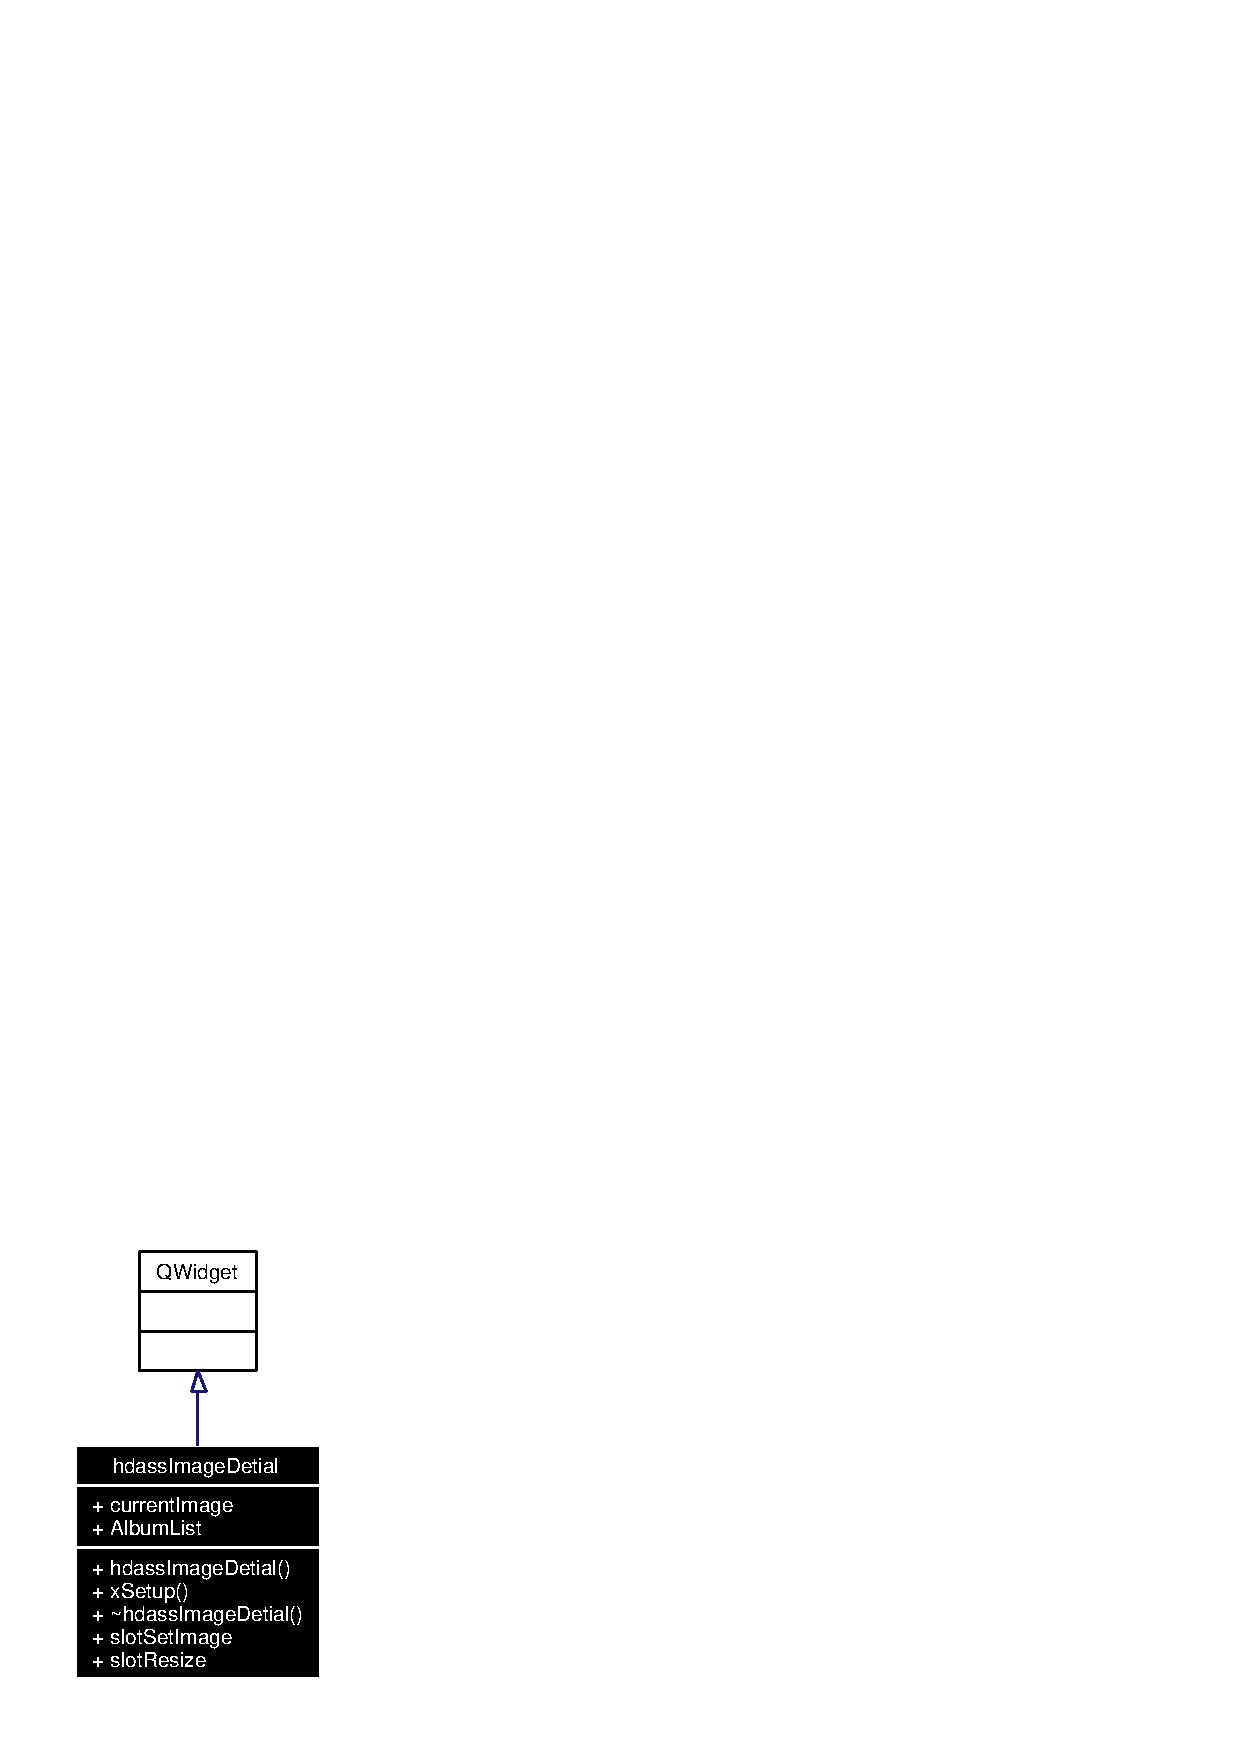
\includegraphics[width=77pt]{classhdassImageDetial__inherit__graph}
\end{center}
\end{figure}
Collaboration diagram for hdass\-Image\-Detial:\begin{figure}[H]
\begin{center}
\leavevmode
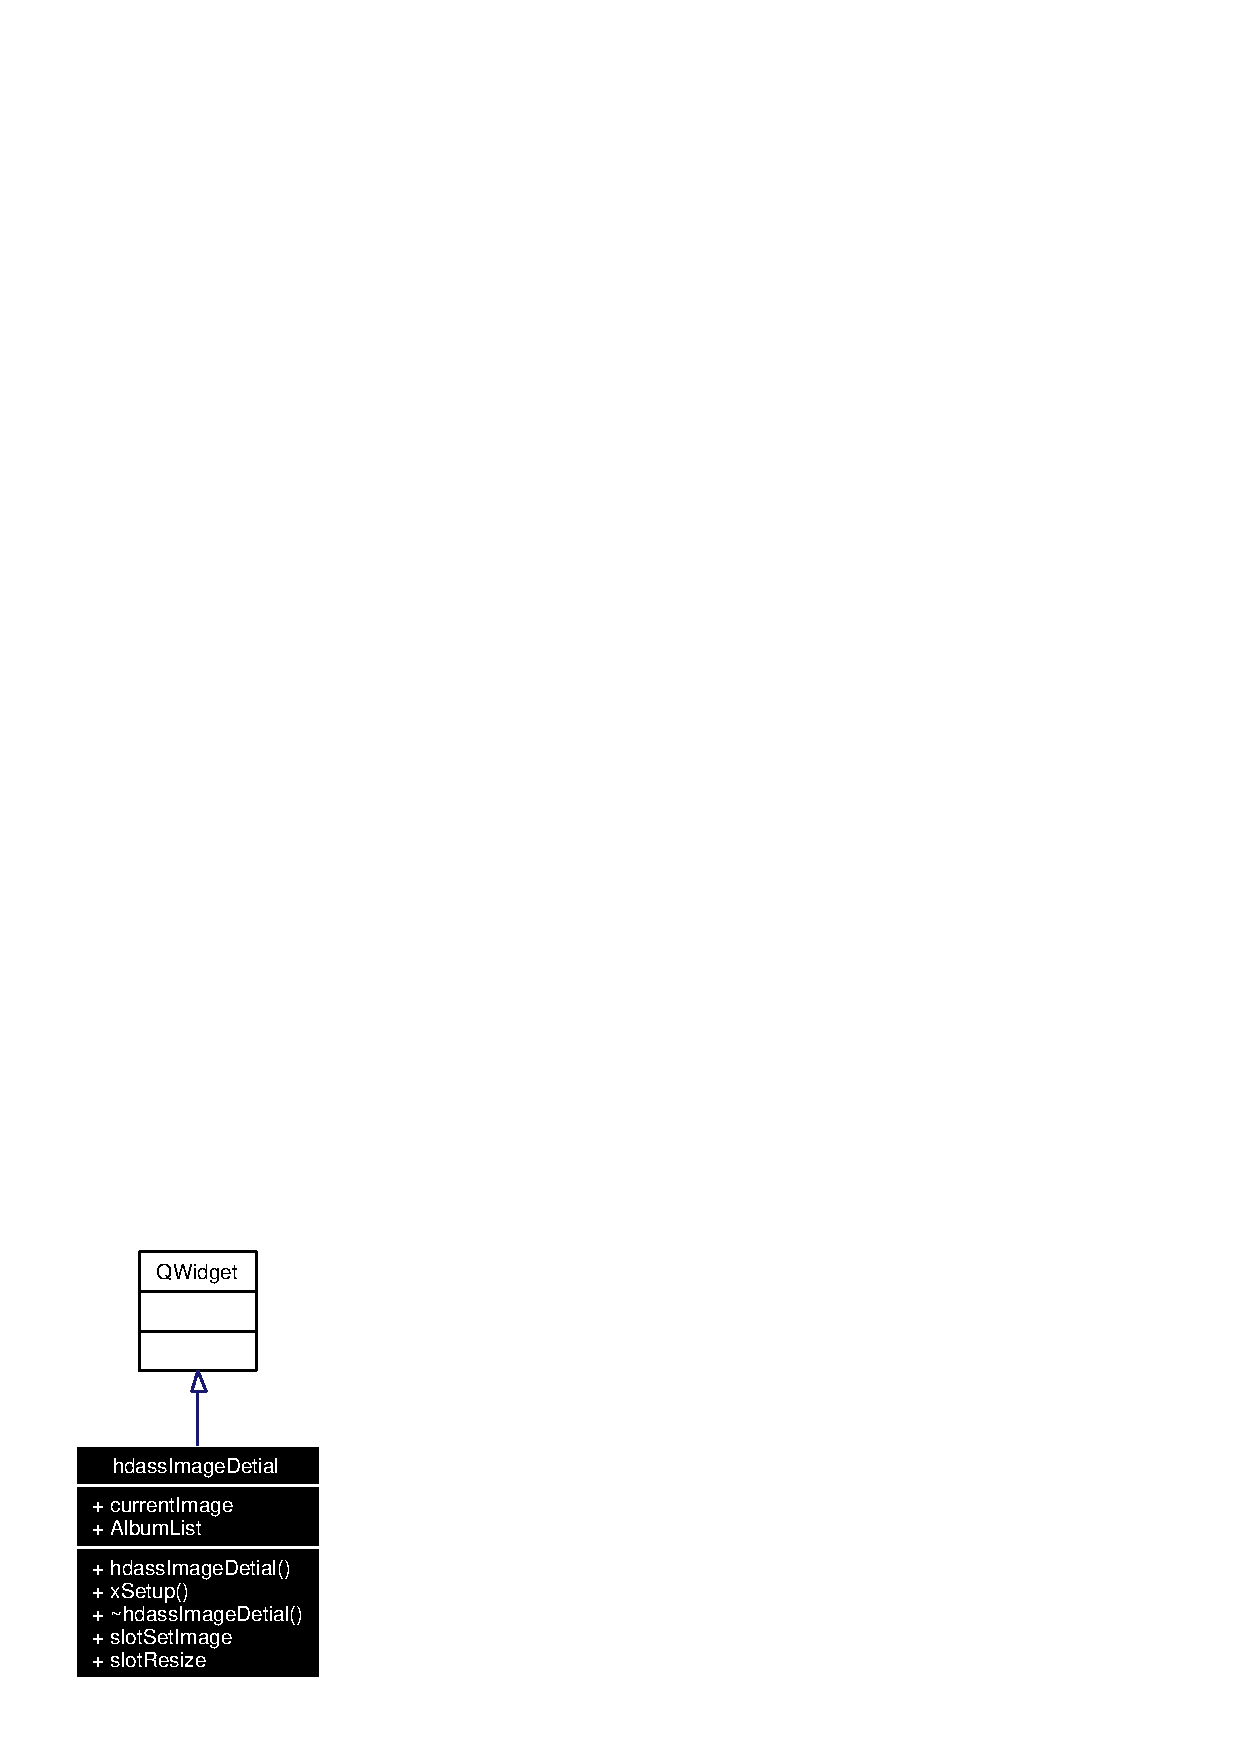
\includegraphics[width=77pt]{classhdassImageDetial__coll__graph}
\end{center}
\end{figure}


\subsection{Detailed Description}
\begin{Desc}
\item[Author:]root \end{Desc}




Definition at line 30 of file hdassimagedetial.h.\subsection*{Public Slots}
\begin{CompactItemize}
\item 
void {\bf slot\-Set\-Image} (KURL url)
\item 
void {\bf slot\-Resize} (int wdith, int height)
\end{CompactItemize}
\subsection*{Public Member Functions}
\begin{CompactItemize}
\item 
{\bf hdass\-Image\-Detial} ({\bf QWidget} $\ast$parent=0, const char $\ast$name=0)
\item 
void {\bf x\-Setup} ()
\item 
{\bf $\sim$hdass\-Image\-Detial} ()
\end{CompactItemize}
\subsection*{Public Attributes}
\begin{CompactItemize}
\item 
QPixmap {\bf current\-Image}
\item 
QPtr\-List$<$ QPixmap $>$ {\bf Album\-List}
\end{CompactItemize}


\subsection{Constructor \& Destructor Documentation}
\index{hdassImageDetial@{hdass\-Image\-Detial}!hdassImageDetial@{hdassImageDetial}}
\index{hdassImageDetial@{hdassImageDetial}!hdassImageDetial@{hdass\-Image\-Detial}}
\subsubsection{\setlength{\rightskip}{0pt plus 5cm}hdass\-Image\-Detial::hdass\-Image\-Detial ({\bf QWidget} $\ast$ {\em parent} = 0, const char $\ast$ {\em name} = 0)}\label{classhdassImageDetial_hdassImageDetiala0}




Definition at line 28 of file hdassimagedetial.cpp.

References x\-Setup().



\footnotesize\begin{verbatim}29  : QWidget(parent, name)
30 {
31         xSetup();
32 }
\end{verbatim}\normalsize 


Here is the call graph for this function:\begin{figure}[H]
\begin{center}
\leavevmode
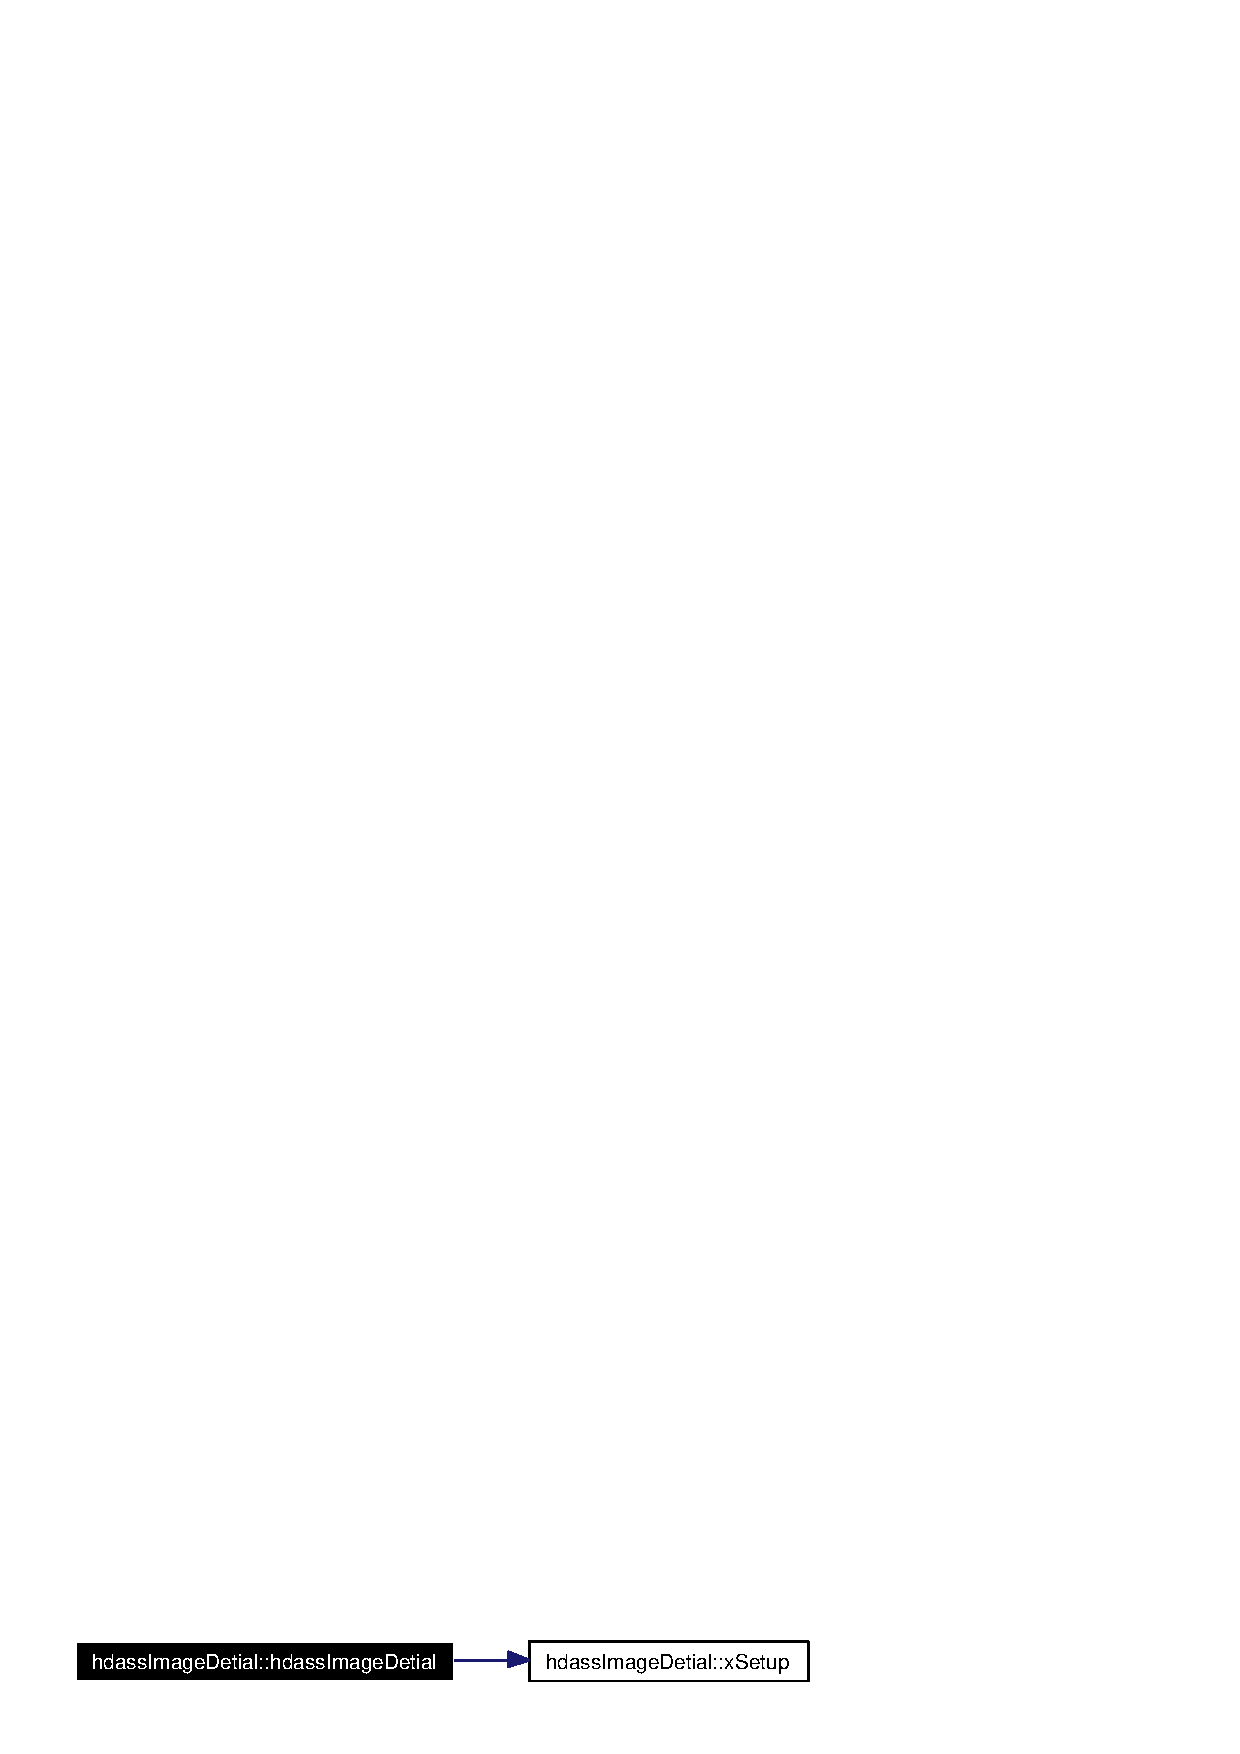
\includegraphics[width=194pt]{classhdassImageDetial_hdassImageDetiala0_cgraph}
\end{center}
\end{figure}
\index{hdassImageDetial@{hdass\-Image\-Detial}!~hdassImageDetial@{$\sim$hdassImageDetial}}
\index{~hdassImageDetial@{$\sim$hdassImageDetial}!hdassImageDetial@{hdass\-Image\-Detial}}
\subsubsection{\setlength{\rightskip}{0pt plus 5cm}hdass\-Image\-Detial::$\sim${\bf hdass\-Image\-Detial} ()}\label{classhdassImageDetial_hdassImageDetiala2}




Definition at line 35 of file hdassimagedetial.cpp.



\footnotesize\begin{verbatim}36 {
37 
38 }
\end{verbatim}\normalsize 


\subsection{Member Function Documentation}
\index{hdassImageDetial@{hdass\-Image\-Detial}!slotResize@{slotResize}}
\index{slotResize@{slotResize}!hdassImageDetial@{hdass\-Image\-Detial}}
\subsubsection{\setlength{\rightskip}{0pt plus 5cm}void hdass\-Image\-Detial::slot\-Resize (int {\em wdith}, int {\em height})\hspace{0.3cm}{\tt  [slot]}}\label{classhdassImageDetial_hdassImageDetiali1}




Definition at line 55 of file hdassimagedetial.cpp.



\footnotesize\begin{verbatim}56 {
57         //resize(width,height);
58 }
\end{verbatim}\normalsize 
\index{hdassImageDetial@{hdass\-Image\-Detial}!slotSetImage@{slotSetImage}}
\index{slotSetImage@{slotSetImage}!hdassImageDetial@{hdass\-Image\-Detial}}
\subsubsection{\setlength{\rightskip}{0pt plus 5cm}void hdass\-Image\-Detial::slot\-Set\-Image (KURL {\em url})\hspace{0.3cm}{\tt  [slot]}}\label{classhdassImageDetial_hdassImageDetiali0}




Definition at line 63 of file hdassimagedetial.cpp.

References current\-Image.



\footnotesize\begin{verbatim}64 {
65 
66    currentImage=QPixmap(url.path());
67    int width ,height;
68    width=currentImage.width();
69    height=currentImage.height();
70    QPixmap draw(QSize(750,330));
71    QPainter p(&draw);
72 
73    p.fillRect(0,0,750,330,Qt::black);
74    if(width<600&&height<330)
75    {
76        //DAVID draw image at center
77        p.drawPixmap((375-width/2),(165-height/2),currentImage);
78    }
79 
80    else
81    {
82         if(11*width>20*height)
83         {
84                 int newheight=(600*height/width);
85                 QImage rescale=currentImage.convertToImage().scale(600,newheight);
86                 p.drawImage(75,165-newheight/2,rescale);
87                 
88         }
89         else
90         {
91                 int newwidth=(330*width/height);
92                 QImage rescale=currentImage.convertToImage().scale(newwidth,330);
93                 p.drawImage((375-newwidth/2),0,rescale);
94         }
95    }    
96    p.end();
97    setBackgroundPixmap(draw);
98 }
\end{verbatim}\normalsize 
\index{hdassImageDetial@{hdass\-Image\-Detial}!xSetup@{xSetup}}
\index{xSetup@{xSetup}!hdassImageDetial@{hdass\-Image\-Detial}}
\subsubsection{\setlength{\rightskip}{0pt plus 5cm}void hdass\-Image\-Detial::x\-Setup ()}\label{classhdassImageDetial_hdassImageDetiala1}




Definition at line 43 of file hdassimagedetial.cpp.

References current\-Image.

Referenced by hdass\-Image\-Detial().



\footnotesize\begin{verbatim}44 {
45    //DAVID Initialize here
46    //DAVID Initial the currentImage with white null pix
47    currentImage=QPixmap(750,330);
48    //set the background image
49    //setBackgroundPixmap(currentImage);
50 }
\end{verbatim}\normalsize 


\subsection{Member Data Documentation}
\index{hdassImageDetial@{hdass\-Image\-Detial}!AlbumList@{AlbumList}}
\index{AlbumList@{AlbumList}!hdassImageDetial@{hdass\-Image\-Detial}}
\subsubsection{\setlength{\rightskip}{0pt plus 5cm}QPtr\-List$<$QPixmap$>$ {\bf hdass\-Image\-Detial::Album\-List}}\label{classhdassImageDetial_hdassImageDetialo1}




Definition at line 38 of file hdassimagedetial.h.\index{hdassImageDetial@{hdass\-Image\-Detial}!currentImage@{currentImage}}
\index{currentImage@{currentImage}!hdassImageDetial@{hdass\-Image\-Detial}}
\subsubsection{\setlength{\rightskip}{0pt plus 5cm}QPixmap {\bf hdass\-Image\-Detial::current\-Image}}\label{classhdassImageDetial_hdassImageDetialo0}




Definition at line 37 of file hdassimagedetial.h.

Referenced by slot\-Set\-Image(), and x\-Setup().

The documentation for this class was generated from the following files:\begin{CompactItemize}
\item 
{\bf hdassimagedetial.h}\item 
{\bf hdassimagedetial.cpp}\end{CompactItemize}
